	La paginación es un método de direccionamiento de memoria
en el cuál se redirigen bloques de direcciones ``virtuales''
a bloques de direcciones físicas. Estos bloques se llaman páginas, y
en la arquitectura intel en el modo usado en el trabajo tiene
un tamaño de 4kb (\texttt{0x1000}). La gran ventaja de la paginación
es que la unidad en la que se trabaja la memoria (la \textit{página})
tiene siempre el mismo tamaño, lo cuál hace que sea fácil hacer manejos
complejos de memoria.

	En la arquitectura intel x86 la paginación se maneja mediante
una estructura de sistema en memoria en 2 niveles. El primer nivel se llama
\textit{page directory} y el segundo \textit{page table}. Los page directory
contienen las direcciones donde se ubican los page table y los page
table contiene direcciones físicas de páginas. De esta manera una dirección
virtual (es decir la dirección a la que accede una tarea) se interpreta
como un índice en el page directory, un índice en la page table obtenida y
, finalmente, un offset para la página encontrada en el page table.

\begin{figure}[h]
\begin{center}
  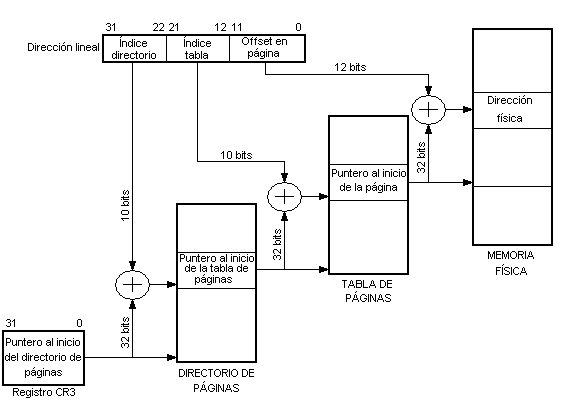
\includegraphics[scale=0.7]{secciones/dibujitos/mmu.png}
\end{center}
\caption{Estructura de paginaci\'on}
\end{figure}

	La siguiente gran ventaja de todo esto es que uno puede tener muchas
estructuras de paginación en memoria y asignarle una distinta a cada tarea.
Esto se hace mediante un registro de control, el \textbf{cr3}. Cuando la
paginación está activa cada vez que se realiza un acceso a memoria
el procesador usa el cr3 para encontrar la dirección del page dir. Modificando
el valor de cr3 se puede hacer que diferentes tareas tengan diferentes \textit{mapas de memoria}
, es decir que cuando accedan a iguales direcciones virtuales lleguen a
diferentes direcciones físicas.

	Si bien mas adelante se va a hablar sobre la seguridad
de manera específica es importante mencionar que debido a que la
segmentación flat detruye todos los sistemas de seguridad que provee
la segmentación la paginación se debe tratar con mucho cuidado, pues
este mecanismo tiene que asegurar toda la seguridad y la integridad de la memoria.

	Además el mapeo de páginas tiene que permitir que las tareas
se ejecuten como si su código estuviera en la posición 1GB (\texttt{0x40000000})
y puedan leer (pero no escribir) desde las direcciones \texttt{0x40002000-0x40002FFF}
direcciones de memoria del kernel.

	Para lograr todo esto implementamos un esquema de paginación en el cuál
existen páginas compartidas y páginas privadas. Pero además existen tablas
de páginas compartidas y tablas de páginas privadas. Además se tuvo especial
cuidado con los permisos otorgados a cada tabla para evitar accesos a memoria
indeseados.

\subsection{Implementación del mapa de memoria}
	El mapa de memoria se inmplementó tal cuál lo dice el enunciado. Hay
identity mapping en los primeros 8mb y después cada tarea tiene
los mapeos que necesita para acceder a su código y al ancla.
	
	En tiempo de ejecución se generan todas las estructuras necesarias
para que el sistema y las tareas puedan funcionar. Esto incluye un page directory para cada
tarea, 1 para el kernel, 1 page table privado de cada tarea (con
permisos de usuario) y 2 page table compartidos(con permisos de administrador).

	Las page table privadas en un principio se inicializan en cero, luego
se actualizan de manera adecuada con funciones de mapeo de página
de las que se hablará mas adelante.

	La otra acción que se realiza en este momento es la de
copiar el código de las tareas de la tierra al mar. Elegimos hacerlo
en este momento porque así ya se pueden hacer los mapeos y dejar
todo todo listo para el momento en que empicen a correr las tareas.

	Todo explicado recién se hacer mediante una sola función escrita en c
que luego se llama desde kernel. asm

	Los page table compartidos tienen los mapeos de las direcciones del kernel.
Esas direcciones estar mapeadas en todas las tareas y con los mismos atributos, motivo
por le cuál decidimos hacerlos comunes. Esto significa todas las primeras entradas
de page dir apuntan al mismo page table, el cuál redirecciona con permisos de administrador
a los primeros 4mb de kernel, del mismo modo todas las segundas entradas
de page dir apuntan también a una page table común que direcciona
a la segunda parte del kernel.


\begin{figure}[h]
\begin{center}
  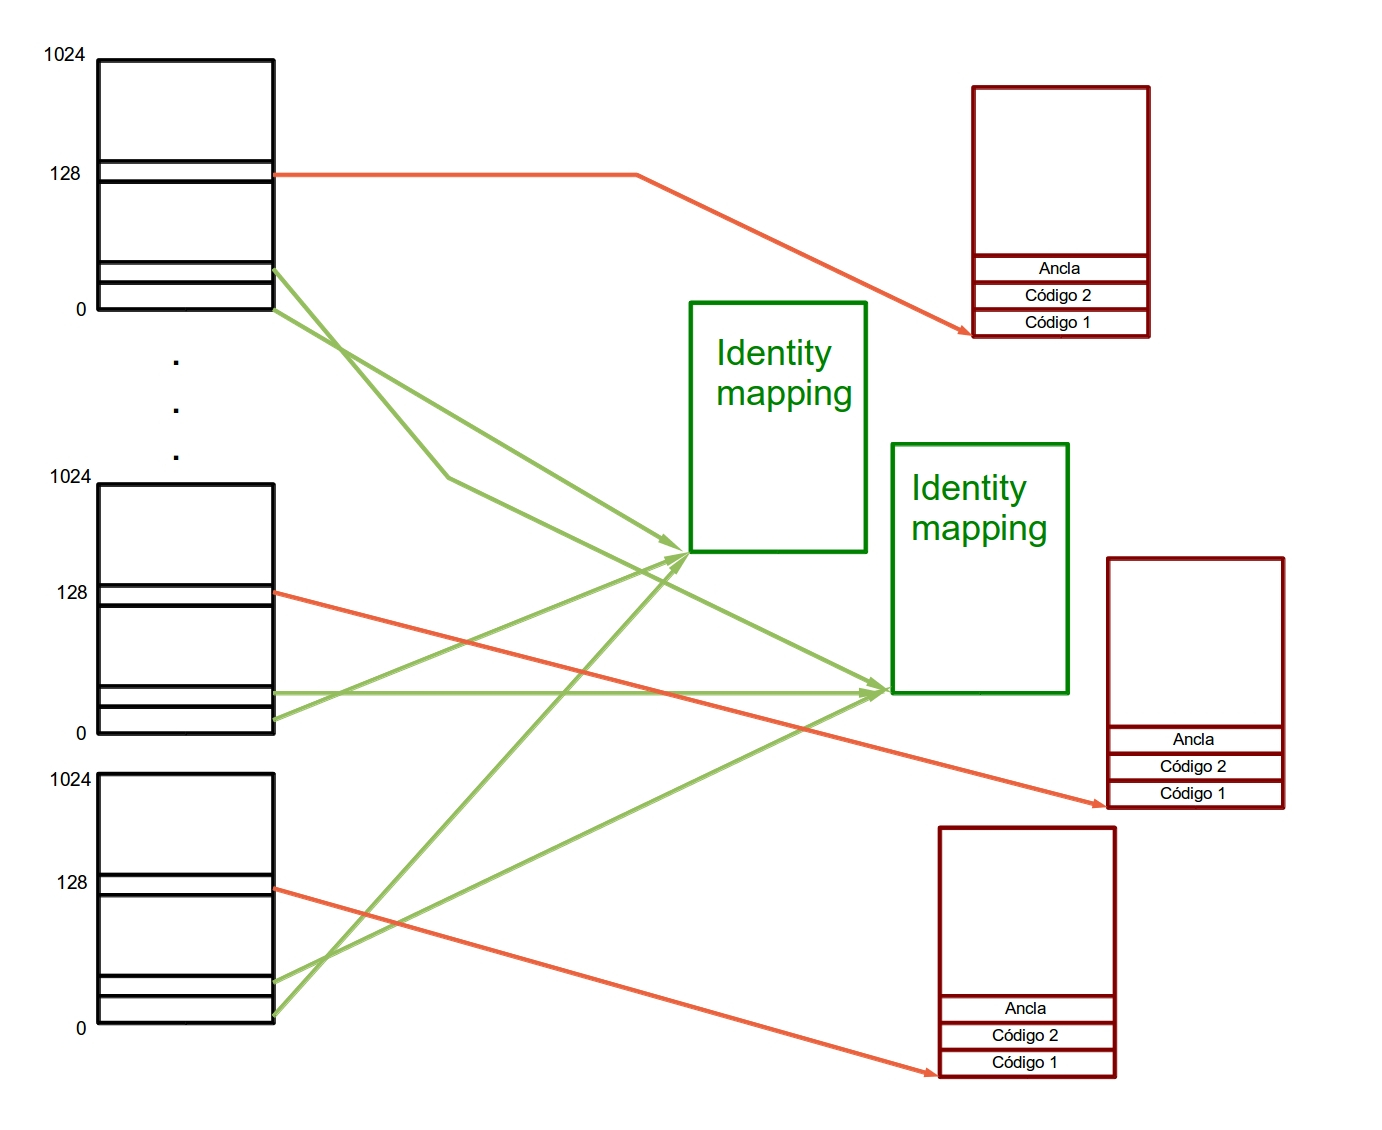
\includegraphics[scale=0.3]{secciones/dibujitos/diagramapaginas.jpg}
\end{center}
\caption{Esquema de las estructuras de paginación}
\label{fig:diagramapaginas}
\end{figure}


	Una vez que el sistema está corriendo los mapeos de página se modifican
en tiempo real mediante dos funciones que se encargan de crear
mapeos de página y de borrar mapeos de página.

\begin{minted}{c}
void mmu_mapear_pagina (unsigned int virtual, unsigned int cr3, unsigned int fisica, unsigned int attr) 
void mmu_unmapear_pagina (unsigned int virtual, unsigned int cr3) 
\end{minted}


	La función encargada de deshacer los mapeos termina con realizando un flush
de la tlb para asegurar la coherencia de todas las estructuras de paginación (
al cambiar un mapeo puede pasar que el mapeo almacenado en la tlb no coincida
más con la realidad).

	Todo esto fue implementado en C. Tanto las funciones
encargadas de crear las estructuras como las funciones encargadas
de los mapeos. Lo único que se hace desde \texttt{kernel.asm} es
llamar a esas funciones en el momento adecuado.

\subsection{Activando la paginación}

	La paginación se activa mediante el bit de paginación, en el
registro \textbf{cr0}. Es indispensable que, en el momento en que se
activa ese bit, cr3 ya esté seteado de manera adecuada y al menos las
estructuras de paginación del kernel esten debidamenta cargadas en memoria.



\begin{comment}
	La parte de paginación se resolvió de manera bastante intuitiva.

	Se crearon funciones en C que se encargar de inicializar los directorios
de páginas del kernel y de las tareas. Un detalle importante de la implementación
es que tanto el kernel como las tareas comparten las primeras 2 tablas de páginas
de sus directores de páginas.

	Estas dos tablas son las que se hacen con identity mapping. El identity mapping
está en todos los mapas de memoria de la misma manera y con los mismos atributos. Además
nunca debe ser cambiado a lo largo de la ejecución de todo el programa en ninguno de los
mapas. Por eso decidimos crear sólo 2 tablas de páginas y hacer que todas las tareas lo compartan.

	En un princio a cada tarea se le asigna una tabla extra inicializada en cero.
Luego mediante las funciones para mapear páginas se completan estas tablas de manera adecuada
para que se efectivicen los mapeos.

	Es importante notar que el resultado final de esto es que cada tarea tiene mapeadas
2 tablas con identity mapping y con proviligios restringidos (sólo para supervisor) y
luego un par de páginas mas con permisos de usuario, que son donde efectivamente va a trabajar.

	Todo eso se englobó en las siguientes funciones de C:
	
\begin{minted}[tabsize=4]{c}
	void mmu_inicializar_dir_kernel();
	void mmu_inicializar_paginas_kernel();
	void mmu_inicializar_tareas();
\end{minted}

	$mmu\_inicializar\_tareas$ no solo inicializar los directorios de páginas sino
que además hace los mapeos de páginas correspondientes.

	Finalmente esas funciones se llaman dentro de kernel.asm. Una vez terminado eso
se habilita la paginación.

\end{comment}
